\documentclass{article}
\usepackage{amsmath}
\usepackage{booktabs}
\usepackage{geometry}
\usepackage{parskip}
\usepackage{tikz}
\usetikzlibrary{positioning, shapes.geometric, arrows}

\geometry{top=0.75in, bottom=0.75in, left=0.75in, right=0.75in}

\title{PERT Analysis for Project Management}
\author{Mahriar Gharaghani - 402672138}
\date{\today}

\begin{document}

\maketitle

\section*{Activity Data}
The table below presents the activities, their respective predecessors, and the duration estimates for each activity in terms of optimistic, pessimistic and probabilistic (most likely) durations:

\begin{tabular}{lccccc}
\toprule
Activity & Predecessors & Optimistic & Pessimistic & Probabilistic \\
\midrule
A & –     & 8  & 14 & 11 \\
B & A     & 7  & 13 & 10 \\
C & B     & 5  & 8  & 6  \\
D & C     & 6  & 12 & 8  \\
E & A     & 9  & 12 & 10 \\
F & B, E  & 7  & 13 & 10 \\
G & C, F  & 8  & 14 & 11 \\
H & D, G  & 10 & 13 & 11 \\
I & E     & 6  & 12 & 9  \\
J & F, I  & 5  & 11 & 9  \\
K & G, J  & 7  & 13 & 10 \\
L & H, K  & 8  & 14 & 11 \\
\bottomrule
\end{tabular}

\vspace{1em} % Add space after the table

\section*{PERT Schedule Table}
The table below shows the calculated values for PERT Scheduling. These values were determined using forward and backward planning.

\begin{tabular}{lcccccccc}
\toprule
Activity & Expected & ES & EF & LS & LF & Slack & Critical & Variance \\
\midrule
A & 11.00 & 0.00 & 11.00 & 0.00 & 11.00 & 0.00 & Yes & 1.00 \\
B & 10.00 & 11.00 & 21.00 & 11.17 & 21.17 & 0.17 & No & 1.00 \\
C & 6.17 & 21.00 & 27.17 & 25.00 & 31.17 & 4.00 & No & 0.25 \\
D & 8.33 & 27.17 & 35.50 & 33.84 & 42.17 & 6.67 & No & 1.00 \\
E & 10.17 & 11.00 & 21.17 & 11.00 & 21.17 & 0.00 & Yes & 0.25 \\
F & 10.00 & 21.17 & 31.17 & 21.17 & 31.17 & 0.00 & Yes & 1.00 \\
G & 11.00 & 31.17 & 42.17 & 31.17 & 42.17 & 0.00 & Yes & 1.00 \\
H & 11.17 & 42.17 & 53.34 & 42.17 & 53.34 & 0.00 & Yes & 0.25 \\
I & 9.00 & 21.17 & 30.17 & 25.67 & 34.67 & 4.50 & No & 1.00 \\
J & 8.67 & 31.17 & 39.84 & 34.67 & 43.34 & 3.50 & No & 1.00 \\
K & 10.00 & 42.17 & 52.17 & 43.34 & 53.34 & 1.17 & No & 1.00 \\
L & 11.00 & 53.34 & 64.34 & 53.34 & 64.34 & 0.00 & Yes & 1.00 \\
\bottomrule
\end{tabular}

\vspace{1em} % Add space after the table

\pagebreak
\section*{Critical Path and Project Duration}
The critical path represents the sequence of activities that determine the project's duration. The activities on the critical path have zero slack, meaning any delay in them will delay the project.

\subsection{Node Diagram}
Below is the Node Diagram representing the activities and their dependencies in the project.

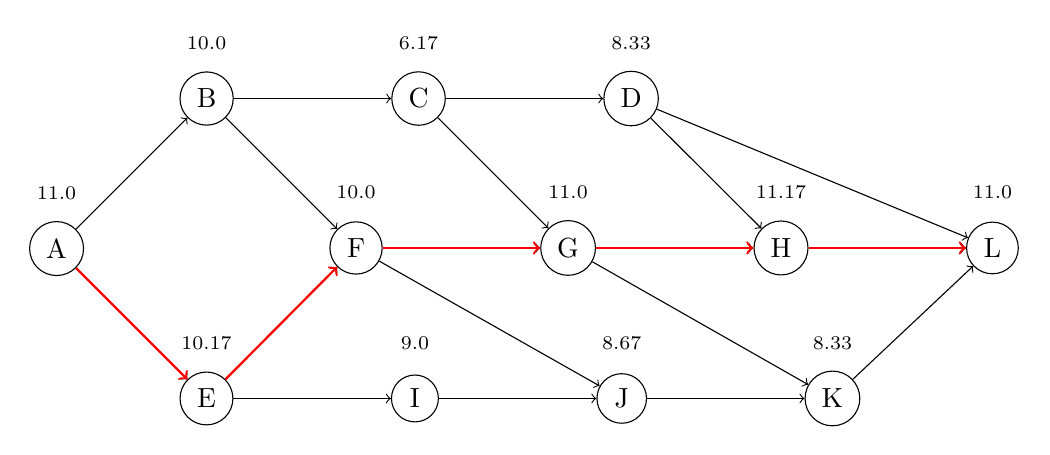
\begin{tikzpicture}[node distance=2cm, auto]
    % Define nodes for activities (Each activity is a circle)
    \node (A) [draw, circle, text centered] {A};
    \node (B) [draw, circle, above right=of A, text centered] {B};
    \node (C) [draw, circle, right=of B, text centered] {C};
    \node (D) [draw, circle, right=of C, text centered] {D};
    \node (E) [draw, circle, below right=of A, text centered] {E};
    \node (F) [draw, circle, below right=of B, text centered] {F};
    \node (G) [draw, circle, right=of F, text centered] {G};
    \node (H) [draw, circle, right=of G, text centered] {H};
    \node (I) [draw, circle, right=of E, text centered] {I};
    \node (J) [draw, circle, right=of I, text centered] {J};
    \node (K) [draw, circle, right=of J, text centered] {K};
    \node (L) [draw, circle, right=of H, text centered] {L};
    
    % Define Expected PERT durations above the nodes
    \node at (A) [above=0.5cm] {\scriptsize 11.0};
    \node at (B) [above=0.5cm] {\scriptsize 10.0};
    \node at (C) [above=0.5cm] {\scriptsize 6.17};
    \node at (D) [above=0.5cm] {\scriptsize 8.33};
    \node at (E) [above=0.5cm] {\scriptsize 10.17};
    \node at (F) [above=0.5cm] {\scriptsize 10.0};
    \node at (G) [above=0.5cm] {\scriptsize 11.0};
    \node at (H) [above=0.5cm] {\scriptsize 11.17};
    \node at (I) [above=0.5cm] {\scriptsize 9.0};
    \node at (J) [above=0.5cm] {\scriptsize 8.67};
    \node at (K) [above=0.5cm] {\scriptsize 8.33};
    \node at (L) [above=0.5cm] {\scriptsize 11.0};
    
    % Draw arrows to indicate dependencies (Edges between nodes)
    \draw[->] (A) -- (B);
    \draw[->] (B) -- (C);
    \draw[->] (C) -- (D);
    \draw[->] (D) -- (H);
    \draw[->] (D) -- (L);
    \draw[->] (A) -- (E);
    \draw[->] (B) -- (F);
    \draw[->] (E) -- (F);
    \draw[->] (F) -- (G);
    \draw[->] (C) -- (G);
    \draw[->] (G) -- (H);
    \draw[->] (E) -- (I);
    \draw[->] (F) -- (J);
    \draw[->] (I) -- (J);
    \draw[->] (G) -- (K);
    \draw[->] (J) -- (K);
    \draw[->] (H) -- (L);
    \draw[->] (K) -- (L);
    
    % Highlight the Critical Path in Red
    \draw[->, red, thick] (H) -- (L);
    \draw[->, red, thick] (A) -- (E);
    \draw[->, red, thick] (E) -- (F);
    \draw[->, red, thick] (F) -- (G);
    \draw[->, red, thick] (G) -- (H);
    
\end{tikzpicture}

\vspace{1em} % Add space after the table

\subsection{Critical Path:} 
\textbf{A → E → F → G → H → L}

The total expected duration of the project is the sum of the expected durations for the activities on the critical path:

\[
\text{Project Expected Duration} = 11.00 + 10.17 + 10.00 + 11.00 + 11.17 + 11.00 = 64.34 \text{ days}
\]

Additionally, we calculate the total variance along the critical path to understand the potential spread of the project’s finish time:

\[
\text{Total Variance} = 1.00 + 0.25 + 1.00 + 1.00 + 0.25 + 1.00 = 4.50
\]

The standard deviation of the project duration can be calculated as:

\[
\sigma = \sqrt{4.50} \approx 2.12 \text{ days}
\]

\vspace{1em} % Add space before the next section

\pagebreak
\section*{Probability Analysis}

\subsection*{Question 1: With 95\% probability, what is the maximum expected project duration?}

To calculate the project duration with 95\% confidence, we use the Z-score for a 95\% confidence level, which is approximately 1.645:

\[
T = \mu + Z \cdot \sigma = 64.34 + (1.645)(2.12) = 67.83 \text{ days}
\]

Therefore, with 95\% probability, the project will finish within \(\boxed{67.83}\) days.

\vspace{1em} % Add space before the next section

\subsection*{Question 2: What is the probability of the project finishing 3 days after the expected finish?}

To find the probability of the project finishing 3 days after the expected finish (i.e., at 67.34 days), we calculate the Z-score for this duration:

\[
Z = \frac{67.34 - 64.34}{2.12} = 1.415
\]

Using standard normal distribution tables, the probability corresponding to a Z-score of 1.415 is approximately 0.9217, or \(92.17\%\).

Thus, the probability of finishing 3 days after the expected finish is approximately \( \boxed{92.17\%} \).




\vspace{1em}

\pagebreak
\section*{Activity on Arrow (AOA) Diagram with Dummy Activities}

The Activity-on-Arrow (AOA) diagram below represents the project’s activities and their dependencies, with dummy activities introduced to maintain logical flow. Dummy activities, depicted as dashed arrows, ensure correct representation of shared dependencies, such as F depending on both B and E. These dummy activities prevent ambiguity in the network structure. They are crucial for preserving the integrity of the project’s dependency relationships. The diagram visually captures the critical path and project timeline.

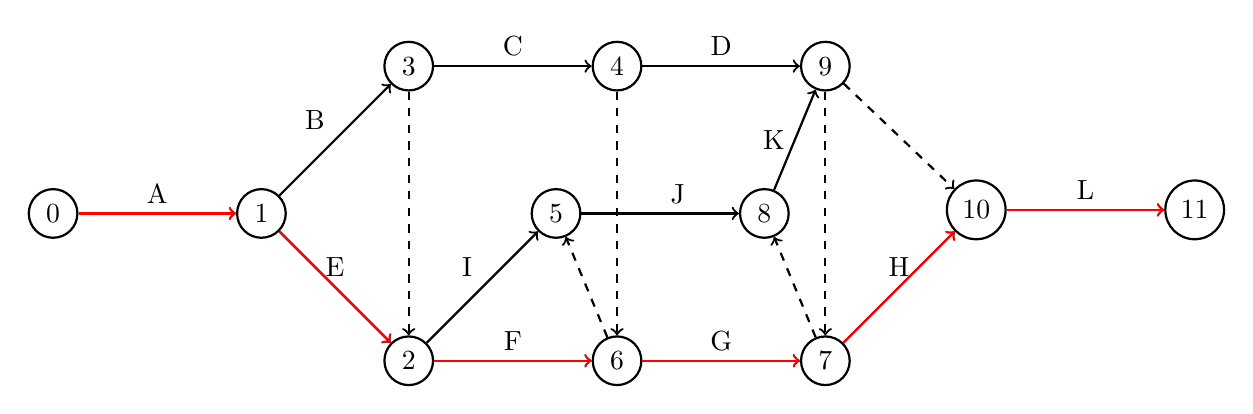
\begin{tikzpicture}[node distance=2cm, auto, thick]
    % Define the event nodes (renumbered)
    \node (E0) [draw, circle, text centered] {0};  % Start Event
    \node (E1) [draw, circle, right=of E0, text centered] {1};  % After A
    \node (E2) [draw, circle, below right=of E1, text centered] {2};  % After E
    \node (E3) [draw, circle, above right=of E1, text centered] {3};  % After B (was 7)
    \node (E4) [draw, circle, right=of E3, text centered] {4};  % After C (was 8)
    \node (E5) [draw, circle, above right=of E2, text centered] {5};  % After I (was 10)
    \node (E6) [draw, circle, right=of E2, text centered] {6};  % After F (was 3)
    \node (E7) [draw, circle, right=of E6, text centered] {7};  % After G (was 4)
    \node (E8) [draw, circle, right=of E5, text centered] {8};  % After J (was 11)
    \node (E9) [draw, circle, right=of E4, text centered] {9};  % After D
    \node (E10) [draw, circle, above right=of E7, text centered] {10};  % After H (was 5)
    \node (E11) [draw, circle, right=of E10, text centered] {11};  % After L / Finish (was 6)

    % Define arrows for activities (unchanged)
    \draw[->] (E0) -- node[above] {A} (E1);
    \draw[->] (E1) -- node[above] {E} (E2);
    \draw[->] (E2) -- node[above] {F} (E6);
    \draw[->] (E6) -- node[above] {G} (E7);
    \draw[->] (E7) -- node[above] {H} (E10);
    \draw[->] (E10) -- node[above] {L} (E11);
    \draw[->] (E1) -- node[above left] {B} (E3);
    \draw[->] (E3) -- node[above] {C} (E4);
    \draw[->] (E4) -- node[above] {D} (E9);
    \draw[->] (E2) -- node[above left] {I} (E5);
    \draw[->] (E5) -- node[above right] {J} (E8);
    \draw[->] (E8) -- node[left] {K} (E9);
    \draw[->, dashed] (E9) -- node[left] {} (E10);  % Dummy to link D+K to H→L
    \draw[->, dashed] (E3) -- node[left] {} (E2);  % Dummy to link D+K to H→L
    \draw[->, dashed] (E4) -- node[left] {} (E6);  % Dummy to link D+K to H→L
    \draw[->, dashed] (E9) -- node[left] {} (E7);  % Dummy to link D+K to H→L
    \draw[->, dashed] (E7) -- node[left] {} (E8);  % Dummy to link D+K to H→L
    \draw[->, dashed] (E6) -- node[left] {} (E5);  % Dummy to link D+K to H→L

    % Highlight the critical path (A → E → F → G → H → L)
    \draw[->, red, thick] (E0) -- (E1);
    \draw[->, red, thick] (E1) -- (E2);
    \draw[->, red, thick] (E2) -- (E6);
    \draw[->, red, thick] (E6) -- (E7);
    \draw[->, red, thick] (E7) -- (E10);
    \draw[->, red, thick] (E10) -- (E11);
\end{tikzpicture}

\end{document}
